%% This is file `elsarticle-template-1-num.tex',
%%
%% Copyright 2009 Elsevier Ltd
%%
%% This file is part of the 'Elsarticle Bundle'.
%% ---------------------------------------------
%%
%% It may be distributed under the conditions of the LaTeX Project Public
%% License, either version 1.2 of this license or (at your option) any
%% later version.  The latest version of this license is in
%%    http://www.latex-project.org/lppl.txt
%% and version 1.2 or later is part of all distributions of LaTeX
%% version 1999/12/01 or later.
%%
%% Template article for Elsevier's document class `elsarticle'
%% with numbered style bibliographic references
%%
%% $Id: elsarticle-template-1-num.tex 149 2009-10-08 05:01:15Z rishi $
%% $URL: http://lenova.river-valley.com/svn/elsbst/trunk/elsarticle-template-1-num.tex $

%%
\documentclass[final,3p,12pt,twocolumn]{elsarticle}


%% Use the option review to obtain double line spacing
%% \documentclass[preprint,review,12pt]{elsarticle}

%% Use the options 1p,twocolumn; 3p; 3p,twocolumn; 5p; or 5p,twocolumn
%% for a journal layout:
%% \documentclass[final,1p,times]{elsarticle}
%% \documentclass[final,1p,times,twocolumn]{elsarticle}
%% \documentclass[final,3p,times]{elsarticle}
%% \documentclass[final,3p,times,twocolumn]{elsarticle}
%% \documentclass[final,5p,times]{elsarticle}
%% \documentclass[final,5p,times,twocolumn]{elsarticle}

%% The graphicx package provides the includegraphics command.
\usepackage{graphicx}
%% The amssymb package provides various useful mathematical symbols
\usepackage{amssymb}
\usepackage[utf8]{inputenc}
%% The amsthm package provides extended theorem environments
%% \usepackage{amsthm}

%% The lineno packages adds line numbers. Start line numbering with
%% \begin{linenumbers}, end it with \end{linenumbers}. Or switch it on
%% for the whole article with \linenumbers after \end{frontmatter}.
\usepackage{lineno}
\usepackage{booktabs}
\usepackage{graphicx}
\usepackage[normalem]{ulem}
\useunder{\uline}{\ul}{}
\usepackage{lscape}
\usepackage{longtable}

\usepackage{pgfplots}
\usepackage{tikz}

\usepackage{float}
\restylefloat{table}

\modulolinenumbers[5]


%% natbib.sty is loaded by default. However, natbib options can be
%% provided with \biboptions{...} command. Following options are
%% valid:

%%   round  -  round parentheses are used (default)
%%   square -  square brackets are used   [option]
%%   curly  -  curly braces are used      {option}
%%   angle  -  angle brackets are used    <option>
%%   semicolon  -  multiple citations separated by semi-colon
%%   colon  - same as semicolon, an earlier confusion
%%   comma  -  separated by comma
%%   numbers-  selects numerical citations
%%   super  -  numerical citations as superscripts
%%   sort   -  sorts multiple citations according to order in ref. list
%%   sort&compress   -  like sort, but also compresses numerical citations
%%   compress - compresses without sorting
%%
%% \biboptions{comma,round}

% \biboptions{}
\usepackage{etoolbox}


\makeatletter

\def\ps@pprintTitle{%
\let\@oddhead\@empty
\let\@evenhead\@empty
\def\@oddfoot{\footnotesize\itshape
% line below modified from elsarticle.cls
 \ifx\@journal\@empty
\else\@journal\fi\hfill\today}%
\let\@evenfoot\@oddfoot}
\makeatother

\begin{document}


\begin{frontmatter}

  %% Title, authors and addresses

  %% use the tnoteref command within \title for footnotes;
  %% use the tnotetext command for the associated footnote;
  %% use the fnref command within \author or \address for footnotes;
  %% use the fntext command for the associated footnote;
  %% use the corref command within \author for corresponding author footnotes;
  %% use the cortext command for the associated footnote;
  %% use the ead command for the email address,
  %% and the form \ead[url] for the home page:
  %%
  %% \title{Title\tnoteref{label1}}
  %% \tnotetext[label1]{}
  %% \author{Name\corref{cor1}\fnref{label2}}
  %% \ead{email address}
  %% \ead[url]{home page}
  %% \fntext[label2]{}
  %% \cortext[cor1]{}
  %% \address{Address\fnref{label3}}
  %% \fntext[label3]{}


  %% use optional labels to link authors explicitly to addresses:
  %% \author[label1,label2]{<author name>}
  %% \address[label1]{<address>}
  %% \address[label2]{<address>}
  \title{\textbf{Systematic Literature Review on Blockchain Oracles} }

  \author[add1]{Pedro Duarte da Costa}
  \ead{pedro.duartecosta@fe.up.pt}
  \author[add1,add2]{Filipe Figueiredo Correia}
  \ead{filipe.correia@fe.up.pt}
  \author[add1,add2]{Hugo Sereno Ferreira}
  \ead{hugosf@fe.up.pt}

  \address[add1]{Faculty of Engineering, University of Porto, Oporto, Portugal}
  \address[add2]{INESC TEC, Oporto, Portugal}

  \begin{abstract}
    Blockchain is fomenting a growing number of solutions and smart contracts are powering new, secure and trusted applications. Smart contracts, currently, lack the important feature of internet connectivity and thus require the use of oracles as a middleware for obtaining information from the Web. This creates a new problem: trusting the use of those oracles; as they do not abide by the same rules as smart contracts. However, current research on Blockchain oracles is scarce and therefore this paper, seeks to systematize existing works regarding oracles, both from academia research as well as from the industry. No survey of the kind was found, to the date of this writing. This analysis comprises a transparent and systematic review of 123 papers queried from the ACM Digital Library, IEEE Xplore, Scopus and Google Scholar. The author concludes that the industry is paving the way in the field of Blockchain oracles and that they can be grouped in the following three categories: \textit{Software-based oracles}, \textit{Hardware-based oracles} and \textit{Consensus-based  oracles}.

  \end{abstract}
  \begin{keyword}
    Blockchain \sep Oracles \sep Trusted Computation
    %% keywords here, in the form: keyword \sep keyword

    %% MSC codes here, in the form: \MSC code \sep code
    %% or \MSC[2008] code \sep code (2000 is the default)
  \end{keyword}



\end{frontmatter}


%\linenumbers

\section{Introduction}

The topic of blockchain oracles is still unexplored territory mostly investigated by start-up companies and individuals thriving to solve a new problem. Therefore, research related to oracles is scarcely found on peer-reviewed publications but, nonetheless, is invaluable in such an early phase of the technology. Consequently, a review on existing work cannot be complete without considering the one developed by academia and also by start-ups, enterprises, governments and individuals.

The goal of this literature review is to get a sense of the corpus of existing works on the topic of blockchain oracles, and the directions and extent to which previous research has rendered significant results.

This review is structured as follows: Section~\ref{sec:2} provides some background knowledge required to clarify important concepts used in the next sections. Section~\ref{sec:3} details the methodology used to carry out the research, including which databases where queried, how they were queried, and the process for including or excluding certain works. Section~\ref{sec:4} analyses further work carried out by the industry. Section~\ref{sec:5} summarises the results found both in academic literature as well as in the industry and answers the first research question. Finally, Section~\ref{sec:6} infers some conclusions on the existing work and answers the second research question.



\section{Background}\label{sec:2}

To discuss the topic of blockchain oracles it's important to understand a few key concepts.

\subsection{Blockchain}
Blockchain is an implementation for distributed consensus, in a byzantine fault-tolerant approach, without requiring to trust in centralized parties. In this ledger, transactions are recorded in an ongoing chain, creating an immutable record.

\subsection{Smart Contracts}
In 2015, Ethereum~\cite{GavinWood2014} was launched as an alternative protocol for building decentralized applications called smart contracts. As applications that run on the blockchain, they are self-verifying, self-executing and immutable contracts whose terms are directly written in lines of code. They can be used to build a wide range of applications.

\subsection{Blockchain Oracles}
Smart contracts lack an important feature: internet connectivity. Due to the deterministic nature of Blockchain and the incompatible indeterministic nature of the Web, smart-contracts cannot directly query it.
Oracles solve the connectivity problem, by listening to events produced by smart contracts, they can insert the needed information on the Blockchain to later be used by the contracts. But oracles do not abide by the same rules and do not support the same guarantees given by Blockchain, so they must either be trusted without hard guarantees about the truthfulness of the data that they provide or we must find ways of guaranteeing their honesty.

\subsection{Authenticity Proofs}
A software or hardware generated cryptographic proof during or after an execution that can later be used to prove the integrity and honesty of the execution or of the provided data.

\subsection{Trusted Execution Environment (TEE)}
A Trusted Execution Environment is a secure computational environment that is strongly isolated from the main operating system. It provides application isolation, integrity and memory confidentiality. Sensitive data is stored, processed and protected from the main operating system or network. This isolation is accomplished through software and hardware-enforced mechanism. TEE runs a small operating system which exposes a minimal interface to the running application and therefore reduces the attack surface. Advanced TEE embeds unique identities that allow to verify the device authenticity and can be used to generate proofs of the device honest execution.

Examples of TEEs are Intel Software Guard Extensions (SGX)~\footnote{More information on Intel SGX can be found here: https://software.intel.com/en-us/sgx/sdk} and ARM Trustzone-based Secure Elements~\citet{Bunz2018}, the latter is commonly found on smartphones. Another example is Trusty~\footnote{More information on Trusty can be found here: https://source.android.com/security/trusty}, a secure Operating System (OS) that provides a TEE for Android. It is isolated from the rest of the system by both hardware and software. Trusty's isolation protects it from malicious apps installed by the user and potential vulnerabilities that may be discovered in Android.


\section{Methodology}\label{sec:3}
A literature review allows scholars not to step on each other's shoes but to climb on each other's shoulders, meaning, not duplicated existing research, find research gaps and strive to discover something new. To conduct a non-biased, methodical and reproducible review we identify its methodology, what are the data sources and what is the selection selection criteria (see \ref{search-process}).

\subsection{Research Questions}
First of all and to guide the focus of the research, the following research questions were defined:
\begin{itemize}
  \item \textbf{RQ1:\label{RQ1} What kind of blockchain oracles have been proposed?}\newline We seek to analyse the scope of existing blockchain oracles. The methodologies and technologies used, so as to understand how the oracle problem is tackled.
  \item \textbf{RQ2:\label{RQ2} What are the research trends on blockchain oracles?}\newline The goal of this question is to identify the main directions of research. Analysing past solutions that never made it into production and solutions currently adopted.
\end{itemize}

\subsection{Search Process}\label{search-process}
Figure \ref{fig:/figures/SLR_stages}, depicts the predefined review strategy that was used. These steps are inspired on the guidelines for performing a systematic review by Kitchenham et al., 2007 \cite{Kitchenham2007}.

\begin{figure*}[h]
  \begin{center}
    \leavevmode
    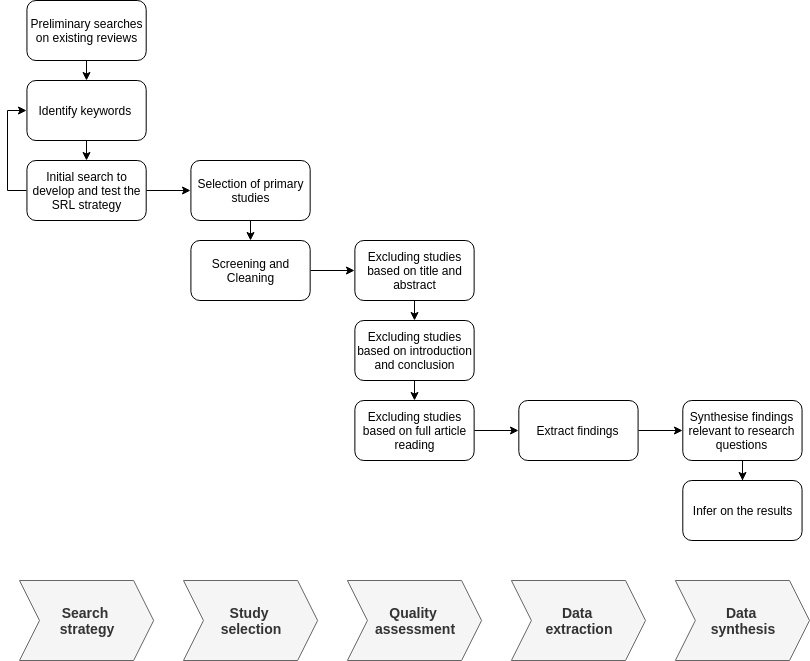
\includegraphics[width=\textwidth]{figures/SLR_stages.png}
    \caption{Systematic Review strategy.}
    \label{fig:/figures/SLR_stages}
  \end{center}
\end{figure*}

The first step, \textbf{Search Strategy and Data-sources}, comprises a preliminary search on several databases trying to optimize the query that best fits the research questions. After identifying the set of keywords that best describe the problem a full query is built and tested.

Once a satisfactory query is achieved, we proceed to the next step, \textbf{Study selection}, here we aggregate the studies from all databases and in the \textit{Screening and cleaning} phase we remove papers written in other languages or duplicated.

Next, in the \textbf{Quality assessment} step we iteratively exclude papers that do not help us answer to any of the research questions. Initially analysing only the title followed by the abstract and so on until a full read of the article seems worth it to take conclusions and respond to que research queries.

This leads to the \textbf{Data extraction} step, in which we take and summarize the findings after reading each paper.

These findings are used in the \textbf{Data synthesis} step, we can summarize all the findings, infer some conclusions and answer the research questions.

\subsection{Search Strategy and Data-sources}
Having defined the strategy for the systematic review and after testing some keywords on several databases, the author selected the following four electronic databases to query for relevant publications:

\begin{itemize}
  \item ACM Digital Library
  \item IEEE Xplore
  \item Scopus
  \item Google Scholar
\end{itemize}

The defined search query was the following:

\texttt{
  (("blockchain" OR "block chain" OR "block-chain")
  AND
  ("oracles" OR "oracle" OR "middle-ware" OR "middleware" OR "middle ware" OR "datafeed" OR "data feed" OR "data-feed"))
}

This search query was used to comprise the most frequent ways of referring to blockchain and oracles. Some scholars have investigated the oracle issue by simply calling them a middleware or data-feed since oracles can either be used as an intermediary that relays data or as the source of the data.

The search was performed on the 5th of February 2019 and revealed the number of results presented in Table \ref{search-results-table}.

\begin{table*}[h]
  \begin{minipage}[c]{\textwidth}
    \centering
    \resizebox{0.7\textwidth}{!}{%
      \begin{tabular}{llr}
        \hline
        \textbf{Database}   & \textbf{Filters}                & \textbf{Results} \\ \hline
        ACM Digital Library & Title, abstract and keywords    & 34               \\
        IEEE Xplore         & Title, abstract and index terms & 24               \\
        Scopus              & Title, abstract and keywords    & 57               \\
        Google Scholar      & Title                           & 8                \\ \hline
        \textbf{Total}      & \textbf{}                       & \textbf{123}     \\ \hline
      \end{tabular}
    }
    \caption{Number of results and applied filters per database}
    \label{search-results-table}
  \end{minipage}
\end{table*}

Since the concept of smart contracts on the blockchain was only introduced in 2015, with the introduction of the Ethereum blockchain~\cite{GavinWood2014}, only results after 2015 were considered, also, all duplicated papers were removed. Analysing the initial search results per year, Figure \ref{search-results-per-year}, we can infer the growing popularity of oracle-related academic research. The year 2019 only comprises work published in the month of January since the search was performed at the beginning of February.

\begin{figure}[H]
  \centering
  \resizebox{0.4\textwidth}{!}{
    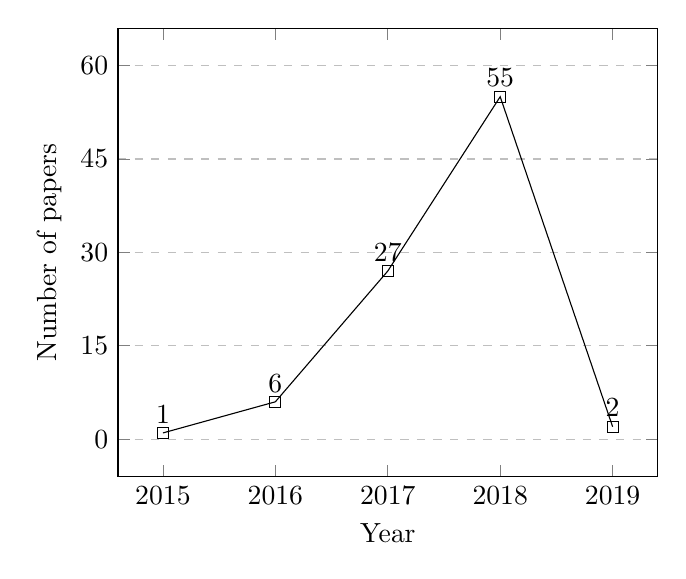
\begin{tikzpicture}
      \begin{axis}[
          xlabel={Year},
          ylabel={Number of papers},
          xtick=data,
          x tick label style={
              /pgf/number format/1000 sep=},
          xmin=2015, xmax=2019,
          ymin=0, ymax=60,
          ytick={0,15,30,45,60,75},
          ymajorgrids=true,
          grid style=dashed,
          enlargelimits=0.10,
        ]

        \addplot[
          mark=square, nodes near coords
        ]
        coordinates {
            (2015,1)(2016,6)(2017,27)(2018,55)(2019,2)
          };

      \end{axis}
    \end{tikzpicture}
  }
  \caption{Resulting papers from search distributed per year}
  \label{search-results-per-year}
\end{figure}

\subsection{Study Selection and Quality Assessment}
The process of exclusion is depicted in Figure \ref{fig:/figures/paper-screening} and all the information regarding the papers and in which phase they were excluded is transparently presented in \ref{ap1:slr}.

The study selection process initially started with a pool of 123 papers from the previously stated online databases. As described on Figure \ref{fig:/figures/SLR_stages}, the selection and quality assessment compromised four stages:
\begin{itemize}
  \item Stage 1: Screening and cleaning duplicated articles or articles that were not in English.
  \item Stage 2: Exclusion by carefully reading the title but most importantly the abstract. After this stage, only 13 of the 91 non-duplicated papers were either describing specific trustable oracle implementations or mentioning the use of oracles.
  \item Stage 3: Analysing the introduction and conclusions in order to remove papers which do not describe an implementation of a trustable oracle or a protocol to overcome the trust in oracles.
  \item Stage 4: Full article reading to assess if the final bucket of articles answers the research questions.
\end{itemize}


\begin{figure}[H]
  \begin{center}
    \leavevmode
    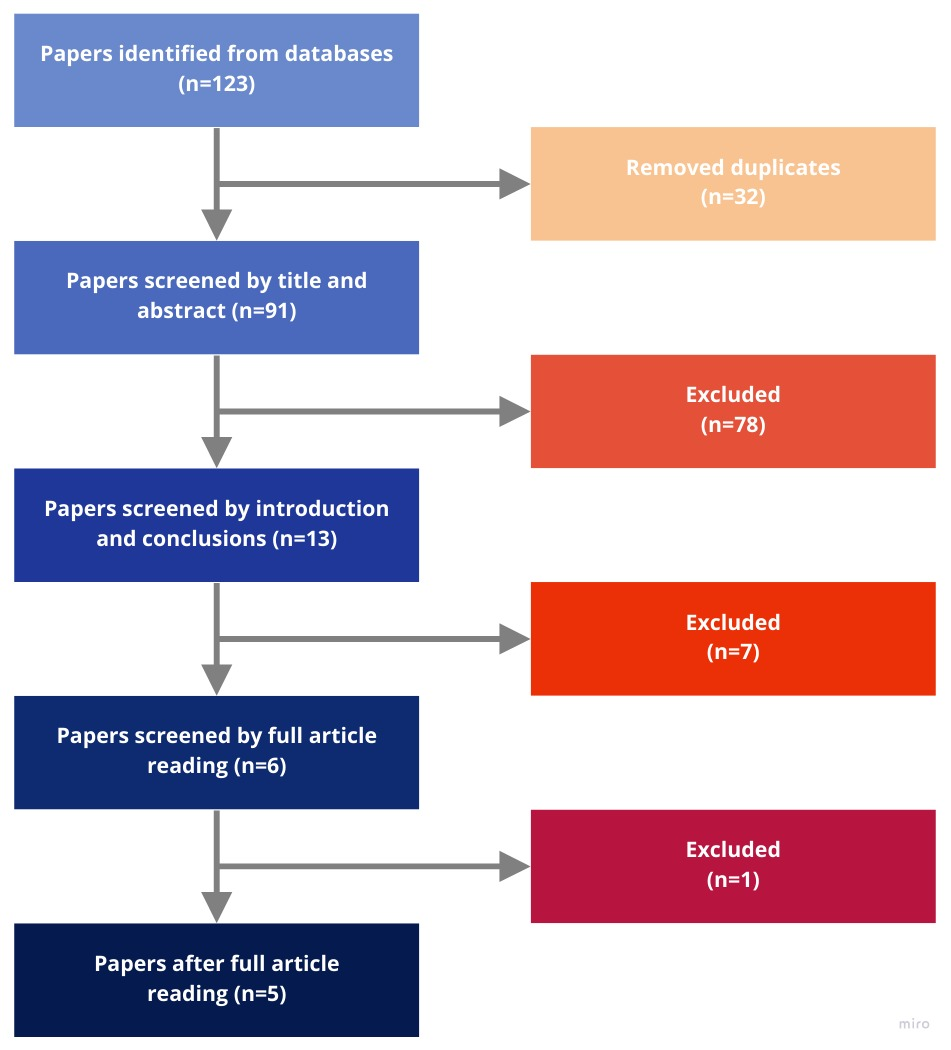
\includegraphics[width=0.5\textwidth]{figures/paper-screening.jpg}
    \caption{Screening stages.}
    \label{fig:/figures/paper-screening}
  \end{center}
\end{figure}


\subsection{Data extraction and Data Synthesis}\label{data-synthesis}

This process resulted in finding three articles and two theses that approach varying problems in implementing and guaranteeing trust in oracles. In these publications the author found the description of eight different implementations or approaches to blockchain oracles, which are analysed in the following paragraphs.

Town Crier (TC) \cite{Zhang2016a}, leverages trusted hardware, specifically Intel SGX\footnote{Intel Corporation. Intel® Software Guard Extensions SDK. https://software.intel.com/en-us/sgx-sdk, 2019}, to scrape HTTPS-enabled websites and serve source-authenticated data to smart contracts. The architecture of TC is depicted on Figure~\ref{fig:/figures/town-crier}~\footnote{Image taken from: https://town-crier.readthedocs.io/en/latest/how\_tc\_works.html}. It involves a TC contract on the blockchain that receives requests from a client contract and communicates those request to a TC server which runs a SGX-protected process to retrieve an answer from a data source through an HTTPS connection. Trusted Execution Environments (TEE) prevent even the operating system of the server from peeking into the enclave or modifying its behaviour, while use of the TLS (Transport Layer Security) protocol prevents tampering or eavesdropping on communications on the network.

\begin{figure}[H]
  \begin{center}
    \leavevmode
    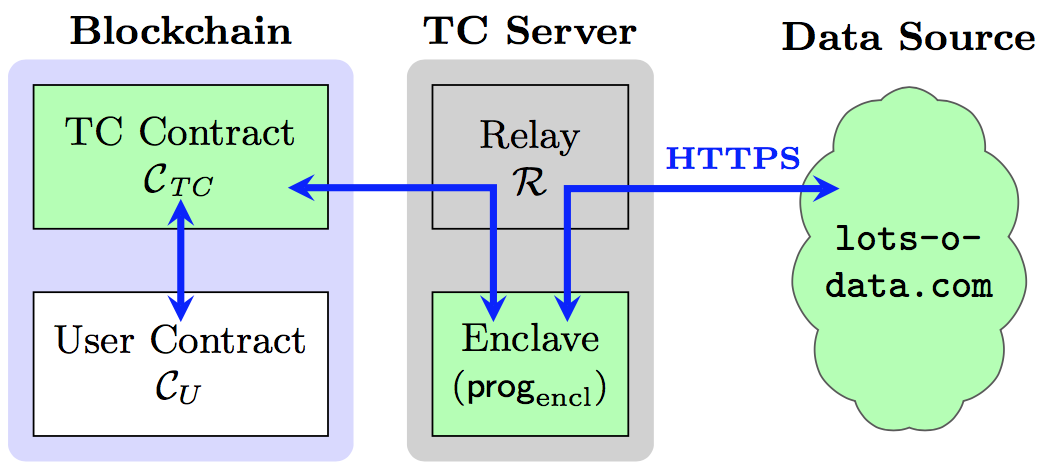
\includegraphics[width=0.45\textwidth]{figures/town-crier.png}
    \caption{Town crier high-level architecture. Figure taken from the Town Crier paper.}
    \label{fig:/figures/town-crier}
  \end{center}
\end{figure}


Astraea, proposed by \citet{Adler2018}, describes a decentralized oracle network, which is depicted on Figure~\ref{fig:/figures/astraea}~\cite{Adler2018a}, with submitters, voters and certifiers, in which voters play a low-risk game and certifiers a high-risk game with associated resources. Using a monetary incentive structure as a means to keep the players honest.

\begin{figure}[H]
  \begin{center}
    \leavevmode
    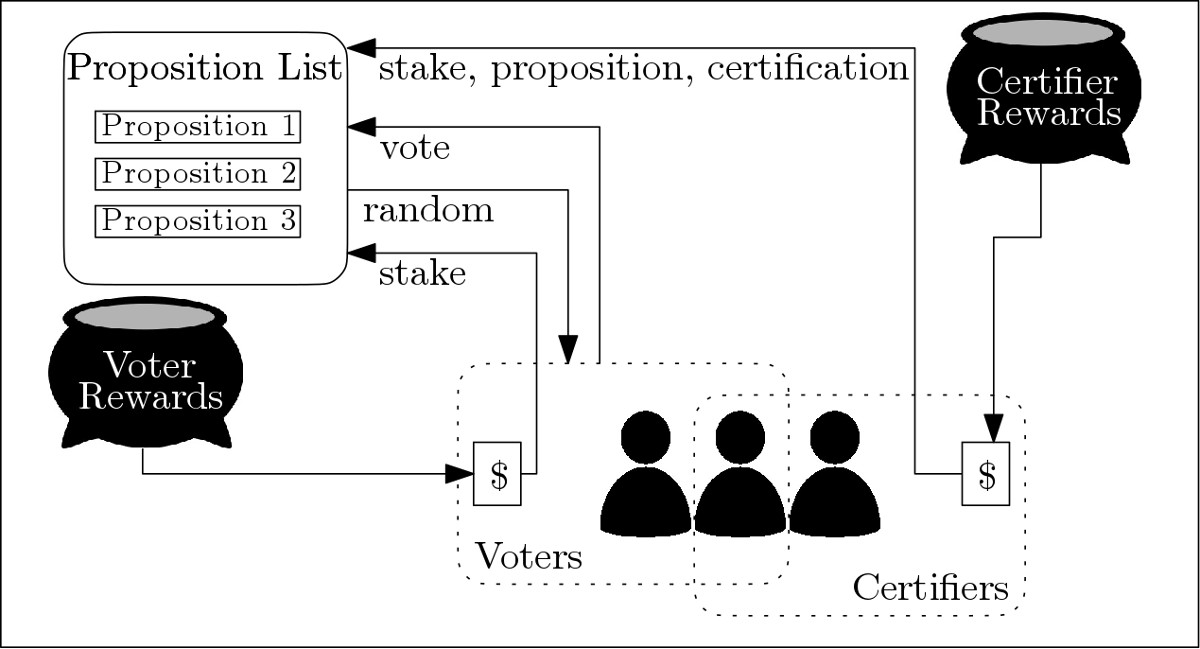
\includegraphics[width=0.45\textwidth]{figures/astraea.jpg}
    \caption{High-level overview of Astraea's architecture.}
    \label{fig:/figures/astraea}
  \end{center}
\end{figure}

Gilroy Gordon \cite{Gordon2017} proposes a protocol for oracle sensor data authenticity and integrity to IoT devices network with low computational resources. Using sets of public and private keys to authenticate that the oracle sensor data actually was originated by that oracle even if the information needs to pass by several oracles before being consumed by the application.

Francisco Monroy \cite{MontotoMonroy2018} defines a gambling protocol based on incentives and assuming that every entity involved has the objective to maximize their profit. The protocol overcomes the trust in a single Oracle by polling a network of 7 oracles from a large network of available oracles, they will then stake their money on a specific bet and only receive their investment back if the majority of the oracles vote in the same winner. Creating, therefore, incentives for Oracle good behaviour.


J. Eberhardt \cite{Eberhardt2018} does not propose a specific method but analyses existing solutions and defines a systematic classification for existing trustable off-chain computation oracles. The authors identify the following off-chain computation oracles approaches:

\begin{itemize}
  \item \textit{Verifiable off-chain Computation}, a technique where a prover executes a computation and then publishes the result including a cryptographic proof attesting the computation’s correctness to the blockchain. An on-chain verifier then verifies the proof and persists the result in case of success. Identified existing solutions are zkSNARKs~\cite{Ben-SassonTechnionAlessandroChiesa2019}, Bulletproofs~\cite{Bunz2018} and zkSTARKs~\cite{Ben-Sasson2018}. zkSNARKs require a setup phase which is more expensive than naive execution. After the setup, however, proof size and verification complexity are extremely small and independent of circuit complexity. This amortization makes zkSNARKs especially efficient for computations executed repeatedly, which is usually the case for off-chain state transitions. While zkSTARKs and Bulletproofs require no setup, proof size and verification complexity grows with circuit complexity, which limits applicability.
  \item \textit{Secure Multiparty Computation}, SMPCs, enable a set of nodes to compute functions on secret data in a way that none of the nodes ever has access to the data in its entirety. Identifies Enigma~\cite{Tam2018}, which proposes a privacy-preserving decentralized computation platform based on multiple parties where a blockchain stores a publicly verifiable audit trail. However, current SMPC protocols add too much overhead for them to be practical. Hence, Enigma now relies on Trusted Execution Environments.
  \item \textit{Enclave-based Computation}, EbC, relying on Trusted Execution Environments (TEE) to execute computations off-chain. Identified existing solutions are Enigma and Ekiden \cite{Cheng2018} which present two different implementations of EbCs. In Enigma, programs can either be executed on-chain or in enclaves that are distributed across a separate off-chain network. An Enigma-specific scripting language allows developers to mark objects as private and hence, enforce off-chain computation. In contrast to Enigma, Ekiden does not allow on-chain computation but instead, the blockchain is solely used as persistent state storage.
  \item \textit{Incentive-driven Off-chain Computation}, IOC, relies on incentive mechanisms applied to motivate off-chain computation and guarantee computational correctness. IOCs inherit two critical design issues: (1) keep verifiers motivated to validate solutions and (2) reduce computational effort for the on-chain judge. The paper identifies TrueBit~\cite{Teutsch2017}, as the first IOC implementation, proposing solutions for both challenges. As verifiers would stop validating if solvers only published correct solutions, TrueBit enforces solvers to provide erroneous solutions from time to time and offers a reward to the verifiers for finding them.
\end{itemize}

\section{Commercial Products and Projects}\label{sec:4}

This search, unlike the systematic one explained before, cannot be described in a systematic way, since the source of the information is scattered throughout whitepapers and documentation webpages of startups, which cannot be guaranteed to be searchable and assessable in a systematic way.

To search for existing commercial products and projects, Google, a search engine and Medium, a platform for blog posting used widely by developers and the start-up community, were used as a means to find new projects or solutions for the oracle trust problem. Using these two tools a lot of projects were found trying to solve the oracle trust problem and are solely documented on white-papers or on the companies' website documentation page. This kind of literature cannot be found in peer-reviewed databases, but can nonetheless provide invaluable information and is therefore worth being analysed.

The results of this search revealed a wide range of projects and protocols with varying degrees of decentralization or authenticity. A short explanation of each will be detailed here:

\begin{itemize}
  \item Oraclize.it \cite{Oraclize.it2018}, provides Authenticity Proofs for the data it fetches guaranteeing that the original data-source is genuine and untampered and can even make use of several data sources in order the gather trustable data, but its centralized model does not guarantee an always available service.
  \item ChainLink\cite{Ellis2017}, describes a decentralized network of oracles that can query multiple sources in order to avoid dependency of a sole oracle, which can be prone to failure and also to gather knowledge from multiple sources to obtain a more reliable result. ChainLink is also considering implementing, in the future, authenticity proofs and make use of trusted hardware, as of now it requires users to trust in the ChainLink nodes to behave correctly.
  \item SchellingCoin~\cite{VitalikButerin2014} protocol incentivizes a decentralized network of oracles to perform computation by rewarding participants who submit results that are closest to the median of all submitted results in a commit-reveal process.
  \item TrueBit~\cite{Teutsch2017}, introduces a system of solvers and verifiers. Solvers are compensated for performing computation and verifiers are compensated for detecting errors in solutions submitted by solvers.
\end{itemize}

\section{Results}\label{sec:5}


\begin{table*}[h]
  \begin{minipage}[c]{\textwidth}
    \centering
    \resizebox{\textwidth}{!}{%
      \begin{tabular}{lccl}
        \hline
        Name                      & Type                       & Distributed Network & Achieves trust through                         \\ \hline
        Town Crier                & Hardware-based             & No                  & Trusted hardware signed attestations           \\
        Astraea                   & Consensus-based            & Yes                 & Network with submitters,  voters and certifier \\
        \citet{Gordon2017}        & Software-based             & Yes                 & Sets of public and private keys                \\
        \citet{MontotoMonroy2018} & Consensus-based            & Yes                 & Gambling protocol based on incentives          \\
        TrueBit                   & Consensus-based            & Yes                 & System of solvers and verifiers                \\
        Oraclize.it               & Software-based             & No                  & TLSNotary, Android Proof                       \\
        ChainLink                 & \begin{tabular}[c]{@{}c@{}}Consensus-based /\\ Software-based\end{tabular} & Yes                 & Query multiple sources                         \\
        SchellingCoin             & Consensus-based            & Yes                 & Incentive based                                \\ \hline
      \end{tabular}
    }
    \caption{Summary of oracle projects/research.}
    \label{oracle-summary}
  \end{minipage}
\end{table*}

A detailed explanation of the findings from the systematic literature search is already detailed in Section~\ref{data-synthesis} and the industry solutions in Section~\ref{sec:4}. This section analyses the combined work from both the academia and industry.

Table \ref{oracle-summary}, summarises the existing projects that were found and answers the first research question (Section \ref{RQ1}) highlighting three main types of oracles.


The first is \textbf{software-based oracles}, which try to prove their honest behaviour through the use of software-based authenticity proofs. These, mostly take advantage of some features of TLS to prove that the data they are relaying is the actually provided data.

The second type is \textbf{hardware-based oracles}. These leverage specific hardware to provide a TEE, to securely separate the environment running the oracle code from the operating system and other applications to achieve higher guarantees on untampered code execution. They may even provide authenticity proofs regarding that the query actually came from a legit TEE.

Lastly, \textbf{consensus-based oracles}, which require a network of peers working together to achieve higher redundancy, having several peers querying the data and even in some cases peers performing the role of the verifier. This last approach largely depends on the existence of such a network and requires the use of monetary incentives to keep the networking running.

The most promising solutions are Town Crier, ChainLink and Oraclize.it .  Town Crier hardware-based solution, more specifically Intel SGX, adds strong guarantees that the computation performed can be trusted due to its isolution from the remaining environment. To this reason, ChainLink is adopting Town Crier\footnote{ChainLink's annoucement regarding the use of Town Crier: https://blog.chain.link/town-crier-and-chainlink/} to add increasing reliability to their distributed solution. The ChainLink distributed oracle network and their partnerships with huge players such as SWIFT~\footnote{SWIFT is a global provider
  of secure financial messaging services, more info: https://www.swift.com/} make it a promising solution, altough a private and fee-based one.

Oraclize.it, is an industry leading service because of their use and research of authenticity proofs. They have also integrations with the most widely used blockchains implementations, such as, Ethereum, EOS~\cite{Block.one2018}, Hyperledger Fabric~\cite{Androulaki}, Rootstock~\footnote{More information on Rootstock can be found here: https://www.rsk.co/} and Corda~\cite{Brown2016}. Their authenticity proofs are both software-based and hardware-based, with the use of TLSNotary~\cite{TLSnotary}, Android Proof~\footnote{More information on the Android Proof can be found here: https://provable.xyz/papers/android\_proof-rev2.pdf} and Ledger Proof~\footnote{More information on the Ledger Proof can be found here: https://docs.provable.xyz/\#security-deepdive-authenticity-proofstypes-ledger-proof}.

In conclusion, the industry presents ready to use solutions for a fee where as the academia mostly investigates the use of consensus-based solutions which adopt an incentives based network. The latter has the problem of requiring such a network of peers to existing in order to be trusted where as the former can be used right away.



\section{Conclusions}\label{sec:6}

In this work, the author surveys 123 papers and fully analyses 5. One resulting in an hardware-based oracle solutions, two consensus-based oracle proposals, one software-based solution for an IoT devices network data authentication and the last one proposing a classification system of existing off-chain computation oracles. The industry presents us four projects, in which two of them are widely in use, namely Oraclize.it and ChainLink, and other two consensus-based solutions. The industry seems to be investing the most on oracle research, as the two previous mentioned companies are developing a wide range of authenticity proofs and leverage hardware solutions to increase their oracles trustability as detailed on the previous section. They are also partnering with major banks and institutions to allow their solutions to power new solutions for smart contracts.

Summarizing, two main conclusions arise from both academic and non-academic research, and answer the second research question \ref{RQ2}.

First of all, there is a clear lack of academic research on the topic of creating trustable oracles. This is mostly likely due to the specificity of the problem and that blockchain related technology is usually paved by start ups and enthusiasts and not yet addressed in universities curricular plans.

Secondly, even though the main research on trustable oracles is being pursued by startups or sole developers all the existing projects seem to be specific to specific blockchain platforms or in very early phases and not yet ready to be generally adopted.

\nolinenumbers
%% The Appendices part is started with the command \appendix;
%% appendix sections are then done as normal sections
%% \appendix

%% \section{}
%% \label{}

%% References
%%
%% Following citation commands can be used in the body text:
%% Usage of \cite is as follows:
%%   \cite{key}          ==>>  [#]
%%   \cite[chap. 2]{key} ==>>  [#, chap. 2]
%%   \cite{key}         ==>>  Author [#]

%% References with bibTeX database:

\bibliographystyle{model1-num-names}
\bibliography{references.bib}

\appendix
\chapter{SLR Screening Stages} \label{ap1:slr}

% Please add the following required packages to your document preamble:
% \usepackage{booktabs}
% \usepackage[normalem]{ulem}
% \useunder{\uline}{\ul}{}
% \usepackage{lscape}
% \usepackage{longtable}
% Note: It may be necessary to compile the document several times to get a multi-page table to line up properly
\begin{landscape}
    \begin{longtable}{
        @{}
        p{1cm}
        p{1cm}
        p{1cm}
        p{1.7cm}
        p{1.5cm}
        p{1cm}
        p{8cm}
        p{6.5cm}
        @{}
        }
    \toprule
    3rd screen & 2nd screen & 1st Screen & Remove Duplicates & Source & Year & Title & Authors \\* \midrule
    \endfirsthead
    %
    \multicolumn{8}{c}%
    {{\bfseries Table \thetable\ continued from previous page}} \\
    \toprule
    3rd screen & 2nd screen & 1st Screen & Remove Duplicates & Source & Year & Title & Authors \\* \midrule
    \endhead
    %
    \bottomrule
    \endfoot
    %
    \endlastfoot
    %
     &  &  & Duplicate & ACM & 2016 & Weaver: A High-performance, Transactional Graph Database Based on Refinable Timestamps & Ayush Dubey and Greg D. Hill and Robert Escriva and Emin G\&\#252;n Sirer \\
     &  &  & Duplicate & ACM & 2016 & Town Crier: An Authenticated Data Feed for Smart Contracts & Fan Zhang and Ethan Cecchetti and Kyle Croman and Ari Juels and Elaine Shi \\
     &  &  & Duplicate & ACM & 2016 & Proof of Luck: An Efficient Blockchain Consensus Protocol & Mitar Milutinovic and Warren He and Howard Wu and Maxinder Kanwal \\
     &  &  & Duplicate & ACM & 2017 & PlaTIBART: A Platform for Transactive IoT Blockchain Applications with Repeatable Testing & Michael A. Walker and Abhishek Dubey and Aron Laszka and Douglas C. Schmidt \\
     &  &  & Duplicate & ACM & 2018 & Ouroboros Genesis: Composable Proof-of-Stake Blockchains with Dynamic Availability & Christian Badertscher and Peter Ga\&\#382;i and Aggelos Kiayias and Alexander Russell and Vassilis Zikas \\
     &  &  & Duplicate & ACM & 2017 & On the Design of Communication and Transaction Anonymity in Blockchain-based Transactive Microgrids & Jonatan Bergquist and Aron Laszka and Monika Sturm and Abhishek Dubey \\
     &  &  & Duplicate & ACM & 2017 & FruitChains: A Fair Blockchain & Rafael Pass and Elaine Shi \\
     &  &  & Duplicate & ACM & 2018 & ContractFuzzer: Fuzzing Smart Contracts for Vulnerability Detection & Bo Jiang and Ye Liu and W. K. Chan \\
     &  &  & Duplicate & ACM & 2016 & Bringing Secure Bitcoin Transactions to Your Smartphone & Davide Frey and Marc X. Makkes and Pierre-Louis Roman and Fran\&\#231;ois Ta\&\#239;ani and Spyros Voulgaris \\
     &  &  & Duplicate & ACM & 2017 & Blackchain: Scalability for Resource-constrained Accountable Vehicle-to-x Communication & Rens W. van der Heijden and Felix Engelmann and David M\&\#246;dinger and Franziska Sch\&\#246;nig and Frank Kargl \\
     &  &  & Duplicate & ACM & 2017 & A General Framework for Blockchain Analytics & Massimo Bartoletti and Stefano Lande and Livio Pompianu and Andrea Bracciali \\
     &  &  & Duplicate & ACM & 2017 & EPBC: Efficient Public Blockchain Client for Lightweight Users & Lei Xu and Lin Chen and Zhimin Gao and Shouhuai Xu and Weidong Shi \\
     &  &  & Duplicate & ACM & 2016 & Blockchains and the Logic of Accountability: Keynote Address & Maurice Herlihy and Mark Moir \\
     &  &  & Duplicate & ACM & 2017 & A Byzantine Fault-tolerant Ordering Service for the Hyperledger Fabric Blockchain Platform & Alysson Bessani and Jo\&\#227;o Sousa and Marko Vukoli\&\#263; \\
     &  &  & Duplicate & IEEE & 2018 & Zero-Trust Hierarchical Management in IoT & M. Samaniego; R. Deters \\
     &  &  & Duplicate & IEEE & 2018 & Secure Pub-Sub: Blockchain-Based Fair Payment With Reputation for Reliable Cyber Physical Systems & Y. Zhao; Y. Li; Q. Mu; B. Yang; Y. Yu \\
     &  &  & Duplicate & IEEE & 2018 & Secure Attribute-Based Signature Scheme With Multiple Authorities for Blockchain in Electronic Health Records Systems & R. Guo; H. Shi; Q. Zhao; D. Zheng \\
     &  &  & Duplicate & IEEE & 2018 & Privacy Improvement Architecture for IoT & E. Kak; R. Orji; J. Pry; K. Sofranko; R. Lomotey; R. Deters \\
     &  &  & Duplicate & IEEE & 2018 & Distributed Solar Self-Consumption and Blockchain Solar Energy Exchanges on the Public Grid Within an Energy Community & C. Plaza; J. Gil; F. de Chezelles; K. A. Strang \\
     &  &  & Duplicate & IEEE & 2018 & Confidential Business Process Execution on Blockchain & B. Carminati; C. Rondanini; E. Ferrari \\
     &  &  & Duplicate & IEEE & 2018 & ChainFS: Blockchain-Secured Cloud Storage & Y. Tang; Q. Zou; J. Chen; K. Li; C. A. Kamhoua; K. Kwiat; L. Njilla \\
     &  &  & Duplicate & IEEE & 2018 & Blockchain-Based IoT-Cloud Authorization and Delegation & N. Tapas; G. Merlino; F. Longo \\
     &  &  & Duplicate & IEEE & 2017 & Blockchain world - Do you need a blockchain? This chart will tell you if the technology can solve your problem & M. E. Peck \\
     &  &  & Duplicate & IEEE & 2018 & Blockchain as a Platform for Secure Inter-Organizational Business Processes & B. Carminati; E. Ferrari; C. Rondanini \\
     &  &  & Duplicate & IEEE & 2018 & Analysis of Security in Blockchain: Case Study in 51\%-Attack Detecting & C. Ye; G. Li; H. Cai; Y. Gu; A. Fukuda \\
     &  &  & Duplicate & IEEE & 2018 & An ID-Based Linearly Homomorphic Signature Scheme and Its Application in Blockchain & Q. Lin; H. Yan; Z. Huang; W. Chen; J. Shen; Y. Tang \\
     &  &  & Duplicate & IEEE & 2019 & A New Lattice-Based Signature Scheme in Post-Quantum Blockchain Network & C. Li; X. Chen; Y. Chen; Y. Hou; J. Li \\
     &  &  & Duplicate & Scopus & 2017 & Towards an economic analysis of routing in payment channel networks & Engelmann, F., Kopp, H., Kargl, F., Glaser, F., Weinhardt, C. \\
     &  &  & Duplicate & Scopus & 2018 & 13th EAI International Conference on Security and Privacy in Communication Networks, SecureComm 2017 & {[}No author name available{]} \\
     &  &  & Duplicate & Scopus & 2017 & VIBES: Fast blockchain simulations for large-scale peer-to-peer networks & Stoykov, L., Zhang, K., Jacobsen, H.-A. \\
     &  &  & Duplicate & Scopus & 2017 & HyperPubSub: a decentralized, permissioned, publish/subscribe service using blockchains & Zupan, N., Zhang, K., Jacobsen, H.-A. \\
     &  &  & Duplicate & Scopus & 2018 & Blockchain as a platform for secure inter-organizational business processes & Carminati, B., Ferrari, E., Rondanini, C. \\
     &  & - &  & ACM & 2017 & Towards an Economic Analysis of Routing in Payment Channel Networks & Felix Engelmann and Henning Kopp and Frank Kargl and Florian Glaser and Christof Weinhardt \\
     &  & - &  & ACM & 2017 & VIBES: Fast Blockchain Simulations for Large-scale Peer-to-peer Networks: Demo & Lyubomir Stoykov and Kaiwen Zhang and Hans-Arno Jacobsen \\
     &  & - &  & ACM & 2018 & StreamChain: Do Blockchains Need Blocks? & Zsolt Istv\&\#225;n and Alessandro Sorniotti and Marko Vukoli\&\#263; \\
     &  & - &  & ACM & 2018 & Sol2Js: Translating Solidity Contracts into Javascript for Hyperledger Fabric & Muhammad Ahmad Zafar and Falak Sher and Muhammad Umar Janjua and Salman Baset \\
     &  & - &  & ACM & 2018 & Scaling Byzantine Consensus: A Broad Analysis & Christian Berger and Hans P. Reiser \\
     &  & - &  & ACM & 2018 & Resource Fairness and Prioritization of Transactions in Permissioned Blockchain Systems (Industry Track) & Seep Goel and Abhishek Singh and Rachit Garg and Mudit Verma and Praveen Jayachandran \\
     &  & - &  & ACM & 2018 & Powering Software Sustainability with Blockchain & Omar Badreddin \\
     &  & - &  & ACM & 2017 & Hyperpubsub: A Decentralized, Permissioned, Publish/Subscribe Service Using Blockchains: Demo & Nejc Zupan and Kaiwen Zhang and Hans-Arno Jacobsen \\
     &  & - &  & ACM & 2017 & How Blockchains Can Help Legal Metrology & Wilson S. Melo,Jr and Alysson Bessani and Luiz F. R. C. Carmo \\
     &  & - &  & ACM & 2018 & eVIBES: Configurable and Interactive Ethereum Blockchain Simulation Framework & Aditya Deshpande and Pezhman Nasirifard and Hans-Arno Jacobsen \\
     &  & - &  & ACM & 2018 & EVA: Fair and Auditable Electric Vehicle Charging Service Using Blockchain & Jelena Pajic and Jos\&\#233; Rivera and Kaiwen Zhang and Hans-Arno Jacobsen \\
     &  & - &  & ACM & 2018 & Deconstructing Blockchains: Concepts, Systems, and Insights & Kaiwen Zhang and Roman Vitenberg and Hans-Arno Jacobsen \\
     &  & - &  & ACM & 2018 & CIDDS: A Configurable and Distributed DAG-based Distributed Ledger Simulation Framework & Mohamed Riswan Abdul Lathif and Pezhman Nasirifard and Hans-Arno Jacobsen \\
     &  & - &  & ACM & 2018 & Blockchains for Business Process Management - Challenges and Opportunities &  \\
     &  & - &  & ACM & 2018 & Blockchain Landscape and AI Renaissance: The Bright Path Forward & Hans-Arno Jacobsen and Mohammad Sadoghi and Mohammad Hossein Tabatabaei and Roman Vitenberg and Kaiwen Zhang \\
     &  & - &  & ACM & 2018 & A Federated Low-Power WAN for the Internet of Things & Mehdi Bezahaf and Ga\&\#235;tan Cathelain and Tony Ducrocq \\
     &  & - &  & ACM & 2018 & Authenticated Modular Maps in Haskell & Victor Cacciari Miraldo and Harold Carr and Alex Kogan and Mark Moir and Maurice Herlihy \\
     &  & - &  & ACM & 2018 & Attack and Vulnerability Simulation Framework for Bitcoin-like Blockchain Technologies & Fabian Sch\&\#252;ssler and Pezhman Nasirifard and Hans-Arno Jacobsen \\
     &  & - &  & Google Shoolar & 2017 & Blockchain Oracles–Einsatz der Blockchain-Technologie für Offline-Anwendungen & A Hoppe \\
     &  & - &  & Google Shoolar & 2018 & Blockchain Coupled Oracle Fusion & D Satpathy \\
     &  & - &  & Google Shoolar & 2018 & Blockchain and Consensus from Proofs of Work without Random Oracles & JA Garay, A Kiayias, G Panagiotakos \\
     &  & - &  & Google Shoolar & 2018 & Blockchain across Oracle: Understand the details and implications of the Blockchain for Oracle developers and customers & R van Mölken \\
     &  & - &  & IEEE & 2018 & Understanding Blockchain Technology: The Costs and Benefits of Decentralization &  \\
     &  & - &  & IEEE & 2018 & Towards Application Portability on Blockchains & K. Shudo; R. Kanda; K. Saito \\
     &  & - &  & IEEE & 2017 & Secure one-time biometrie tokens for non-repudiable multi-party transactions & K. Nandakumar; N. Ratha; S. Pankanti; S. Darnell \\
     &  & - &  & IEEE & 2017 & Multiclouds in an Enterprise – a Love-Hate Relationship & M. Yousif \\
     &  & - &  & IEEE & 2019 & Leveraging the Capabilities of Industry 4.0 for Improving Energy Efficiency in Smart Factories & N. Mohamed; J. Al-Jaroodi; S. Lazarova-Molnar \\
     &  & - &  & IEEE & 2017 & Fostering consumers' energy market through smart contracts & I. Kounelis; G. Steri; R. Giuliani; D. Geneiatakis; R. Neisse; I. Nai-Fovino \\
     &  & - &  & IEEE & 2018 & ChainMOB: Mobility Analytics on Blockchain & B. Nasrulin; M. Muzammal; Q. Qu \\
     &  & - &  & IEEE & 2016 & Blockchains and the logic of accountability & M. Herlihy; M. Moir \\
     &  & - &  & IEEE & 2018 & Blockchain Based Security Framework for IoT Implementations & K. N. Krishnan; R. Jenu; T. Joseph; M. L. Silpa \\
     &  & - &  & IEEE & 2018 & Blockchain Based Vehicular Data Management & R. Sharma; S. Chakraborty \\
     &  & - &  & Scopus & 2016 & Weaver: A high-performance, transactional graph database based on refinable timestamps & Dubey, A., Hill, G.D., Sirer, E.G., Escriva, R. \\
     &  & - &  & Scopus & 2018 & Towards a smart contract-based, decentralized, public-key infrastructure & Patsonakis, C., Samari, K., Roussopoulos, M., Kiayias, A. \\
     &  & - &  & Scopus & 2016 & SysTEX 2016 - 1st Workshop on System Software for Trusted Execution, colocated with ACM/IFIP/USENIX Middleware 2016 & {[}No author name available{]} \\
     &  & - &  & Scopus & 2018 & Systematic performance evaluation using component-in-the-loop approach & Kocsis, I., Klenik, A., Pataricza, A., Telek, M., Deé, F., Cseh, D. \\
     &  & - &  & Scopus & 2018 & Synchronized aggregate signatures from the RSA assumption & Hohenberger, S., Waters, B. \\
     &  & - &  & Scopus & 2018 & Simple proofs of sequential work & Cohen, B., Pietrzak, K. \\
     &  & - &  & Scopus & 2017 & SERIAL 2017 - 1st Workshop on Scalable and Resilient Infrastructures for Distributed Ledgers, Colocated with ACM/IFIP/USENIX Middleware 2017 Conference & {[}No author name available{]} \\
     &  & - &  & Scopus & 2018 & Security of the blockchain against long delay attack & Wei, P., Yuan, Q., Zheng, Y. \\
     &  & - &  & Scopus & 2018 & Secure Pub-Sub: Blockchain-Based Fair Payment with Reputation for Reliable Cyber Physical Systems & Zhao, Y., Li, Y., Mu, Q., Yang, B., Yu, Y. \\
     &  & - &  & Scopus & 2018 & Secure Attribute-Based Signature Scheme with Multiple Authorities for Blockchain in Electronic Health Records Systems & Guo, R., Shi, H., Zhao, Q., Zheng, D. \\
     &  & - &  & Scopus & 2017 & RingCT 2.0: A compact accumulator-based (linkable ring signature) protocol for blockchain cryptocurrency Monero & Sun, S.-F., Au, M.H., Liu, J.K., Yuen, T.H. \\
     &  & - &  & Scopus & 2016 & Proof of Luck: An efficient blockchain consensus protocol & Milutinovic, M., He, W., Wu, H., Kanwal, M. \\
     &  & - &  & Scopus & 2018 & Privacy improvement architecture for IoT & Kak, E., Orji, R., Pry, J., Sofranko, K., Lomotey, R.K., Deters, R. \\
     &  & - &  & Scopus & 2017 & PlaTIBART: A Platform for Transactive IoT blockchain applications with repeatable testing & Walker, M.A., Dubey, A., Laszka, A., Schmidt, D.C. \\
     &  & - &  & Scopus & 2017 & Overcoming Cryptographic Impossibility Results Using Blockchains & Goyal, R., Goyal, V. \\
     &  & - &  & Scopus & 2018 & Ouroboros praos: An adaptively-secure, semi-synchronous proof-of-stake blockchain & David, B., Gaži, P., Kiayias, A., Russell, A. \\
     &  & - &  & Scopus & 2017 & On the design of communication and transaction anonymity in blockchain-based transactive microgrids & Bergquist, J., Laszka, A., Sturm, M., Dubey, A. \\
     &  & - &  & Scopus & 2017 & Middleware 2017 - Proceedings of the 2017 Middleware Posters and Demos 2017: Proceedings of the Posters and Demos Session of the 18th International Middleware Conference & {[}No author name available{]} \\
     &  & - &  & Scopus & 2017 & M4IoT 2017 - Proceedings of the 2017 Workshop on Middleware and Applications for the Internet of Things 4th Edition and 2nd Federated Event with the MoTA Workshop, Part of Middleware 2017 Conference & {[}No author name available{]} \\
     &  & - &  & Scopus & 2018 & IoTBDS 2018 - Proceedings of the 3rd International Conference on Internet of Things, Big Data and Security & {[}No author name available{]} \\
     &  & - &  & Scopus & 2018 & Introducing the new paradigm of Social Dispersed Computing: Applications, Technologies and Challenges & García-Valls, M., Dubey, A., Botti, V. \\
     &  & - &  & Scopus & 2017 & FruitChains: A fair blockchain & Pass, R., Shi, E. \\
     &  & - &  & Scopus & 2017 & EPBC: Efficient Public Blockchain Client for Lightweight Users & Xu, L., Chen, L., Gao, Z., Xu, S., Shi, W. \\
     &  & - &  & Scopus & 2018 & Distributed Solar Self-Consumption and Blockchain Solar Energy Exchanges on the Public Grid Within an Energy Community & Plaza, C., Gil, J., De Chezelles, F., Strang, K.A. \\
     &  & - &  & Scopus & 2018 & Designing blockchain-based SIEM 3.0 system & Miloslavskaya, N. \\
     &  & - &  & Scopus & 2018 & ChainFS: Blockchain-Secured Cloud Storage & Tang, Y., Zou, Q., Chen, J., Li, K., Kamhoua, C.A., Kwiat, K., Njilla, L. \\
     &  & - &  & Scopus & 2016 & Bringing secure Bitcoin transactions to your smartphone & Frey, D., Makkes, M.X., Roman, P.-L., Taïani, F., Voulgaris, S. \\
     &  & - &  & Scopus & 2015 & Blockchain-based model for social transactions processing & Sarr, I., Naacke, H., Gueye, I. \\
     &  & - &  & Scopus & 2018 & Blockchain-Based IoT-cloud authorization and delegation & Tapas, N., Merlino, G., Longo, F. \\
     &  & - &  & Scopus & 2017 & Blockchain world - Do you need a blockchain? This chart will tell you if the technology can solve your problem & Peck, M.E. \\
     &  & - &  & Scopus & 2017 & Blackchain: Scalability for resource-constrained accountable vehicle-to-x communication & Van Der Heijden, R.W., Engelmann, F., Mödinger, D., Schönig, F., Kargl, F. \\
     &  & - &  & Scopus & 2017 & Beyond hellman’s time-memory trade-offs with applications to proofs of space & Abusalah, H., Alwen, J., Cohen, B., Khilko, D., Pietrzak, K., Reyzin, L. \\
     &  & - &  & Scopus & 2017 & Analysis of the blockchain protocol in asynchronous networks & Pass, R., Seeman, L., Shelat, A. \\
     &  & - &  & Scopus & 2018 & Analysis of security in blockchain: Case study in 51\%-attack detecting & Ye, C., Li, G., Cai, H., Gu, Y., Fukuda, A. \\
     &  & - &  & Scopus & 2018 & An integrated platform for the Internet of Things based on an open source ecosystem & Li, Y.Q. \\
     &  & - &  & Scopus & 2018 & An ID-Based Linearly Homomorphic Signature Scheme and Its Application in Blockchain & Lin, Q., Yan, H., Huang, Z., Chen, W., Shen, J., Tang, Y. \\
     &  & - &  & Scopus & 2019 & A New Lattice-Based Signature Scheme in Post-Quantum Blockchain Network & Li, C.-Y., Chen, X.-B., Chen, Y.-L., Hou, Y.-Y., Li, J. \\
     &  & - &  & Scopus & 2017 & A general framework for blockchain analytics & Bartoletti, M., Lande, S., Pompianu, L., Bracciali, A. \\
     &  & - &  & Scopus & 2018 & A critical look at cryptogovernance of the real world: Challenges for spatial representation and uncertainty on the blockchain & Adams, B., Tomko, M. \\
     &  & - &  & Scopus & 2017 & A byzantine fault-tolerant ordering service for the hyperledger fabric blockchain platform (Short Paper) & Bessani, A., Sousa, J., Vukolić, M. \\
     &  & - &  & Scopus & 2017 & 4th International Conference on Future Data and Security Engineering, FDSE 2017 & {[}No author name available{]} \\
     &  & - &  & Scopus & 2018 & 3rd International Conference on Internet of Things, ICIOT 2018 Held as Part of the Services Conference Federation, SCF 2018 & {[}No author name available{]} \\
     &  & - &  & Scopus & 2017 & 36th Annual International Conference on the Theory and Applications of Cryptographic Techniques, EUROCRYPT 2017 & {[}No author name available{]} \\
     &  & - &  & Scopus & 2018 & 21 - Bringing down the complexity: Fast composable protocols for card games without secret state & David, B., Dowsley, R., Larangeira, M. \\
     &  & - &  & Scopus & 2018 & 13th EAI International Conference on Security and Privacy in Communication Networks, SecureComm 2017 & {[}No author name available{]} \\
     &  & - &  & Scopus & 2017 & 11th International Conference on Provable Security, ProvSec 2017 & {[}No author name available{]} \\
     & - & pass &  & ACM & 2018 & Towards Solving the Data Availability Problem for Sharded Ethereum & Daniel Sel and Kaiwen Zhang and Hans-Arno Jacobsen \\
     & - & pass &  & Google Shoolar & 2018 & Trusted agent blockchain oracle & MD Jackson \\
     & - & pass &  & IEEE & 2018 & Towards Distributed SLA Management with Smart Contracts and Blockchain & R. B. Uriarte; R. de Nicola; K. Kritikos \\
     & - & pass &  & Scopus & 2018 & Zero-trust hierarchical management in IoT & Samaniego, M., Deters, R. \\
     & - & pass &  & Scopus & 2018 & The interface between blockchain and the real world & Damjan, M. \\
     & - & pass &  & Scopus & 2018 & Ouroboros genesis: Composable proof-of-stake blockchains with dynamic availability & Badertscher, C., Gaži, P., Kiayias, A., Russell, A., Zikas, V. \\
     & - & pass &  & Scopus & 2018 & ContractFuzzer: Fuzzing smart contracts for vulnerability detection & Jiang, B., Liu, Y., Chan, W.K. \\
    - & pass & pass &  & Scopus & 2018 & Confidential Business Process Execution on Blockchain & Carminati, B., Rondanini, C., Ferrari, E. \\
    pass & pass & pass &  & ACM & 2018 & Off-chaining Models and Approaches to Off-chain Computations & Jacob Eberhardt and Jonathan Heiss \\
    pass & pass & pass &  & Google Shoolar & 2018 & Astraea: A decentralized blockchain oracle & J Adler, R Berryhill, A Veneris, Z Poulos, N Veira… \\
    pass & pass & pass &  & Google Shoolar & 2017 & Provenance and authentication of oracle sensor data with block chain lightweight wireless network authentication scheme for constrained oracle sensors & G Gordon \\
    pass & pass & pass &  & Google Shoolar & 2018 & Bitcoin gambling using distributed oracles in the blockchain & FJA Montoto Monroy \\
    pass & pass & pass &  & Scopus & 2016 & Town crier: An authenticated data feed for smart contracts & Zhang, F., Cecchetti, E., Croman, K., Juels, A., Shi, E. \\* \bottomrule
    \end{longtable}
    \end{landscape}

%% Authors are advised to submit their bibtex database files. They are
%% requested to list a bibtex style file in the manuscript if they do
%% not want to use model1-num-names.bst.

%% References without bibTeX database:

% \begin{thebibliography}{00}

%% \bibitem must have the following form:
%%   \bibitem{key}...
%%

% \bibitem{}

% \end{thebibliography}


\end{document}

%%
%% End of file `elsarticle-template-1-num.tex'.